\section{AAr Cryostat}
\label{sec:Cryostat}

Figure~\ref{fig:DSk3D} shows the \DSk\ system conceptual sketch, including the copper electromagnetic and light shield, the Veto detector and the \LArTPC, all contained within the large \AAr\ cryostat.  A \pDUNE-like cryostat will be employed to house the \LAr\ bath which the \TPC\ is immersed in and also acts as the main component of the Veto detector. This allows to minimize the material of the \TPC\ vessel and therefore to limit the possible radio-contaminations very close to the active volume.  

\begin{figure*}[!t]
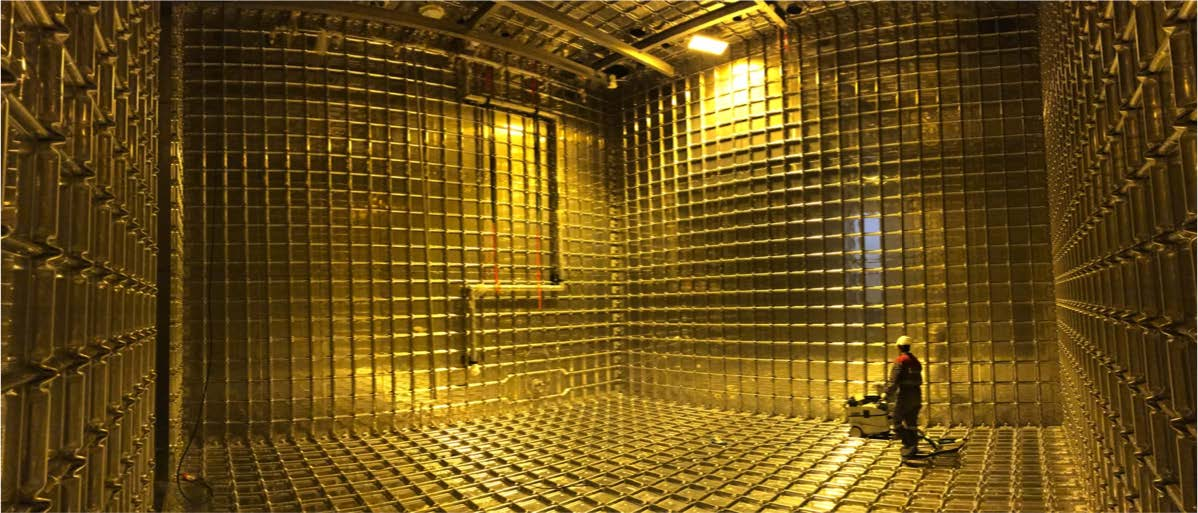
\includegraphics[height=0.30\textwidth]{./Figures/ProtoDUNE-Cryostat-Inner-Photo.jpg}
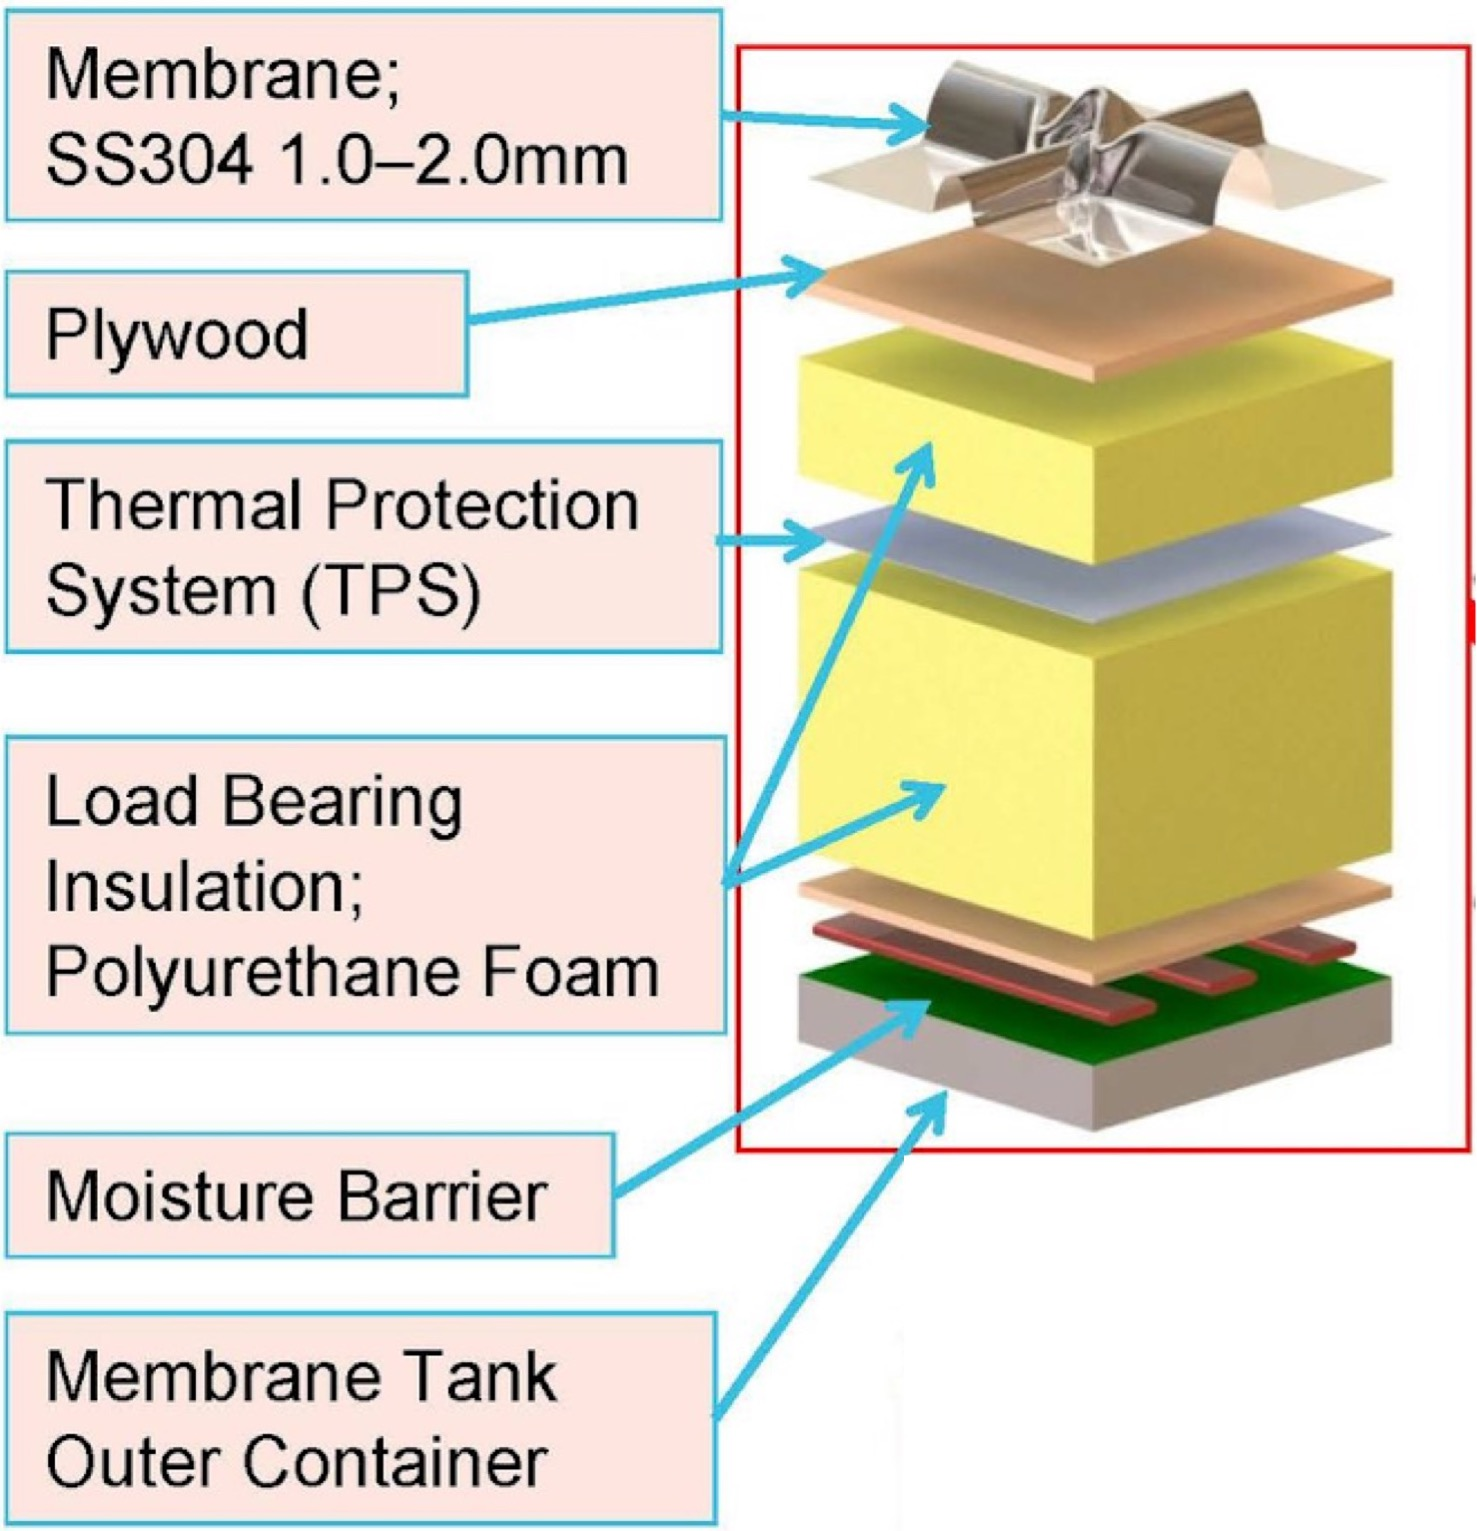
\includegraphics[height=0.30\textwidth]{./Figures/Membrane-concept.jpg}
\caption[Details of the \AAr\ cryostat]{{\bf Left} Interior view of the \pDUNE\ cryostat used for the single phase \LArTPC\ test at \CERN.  {\bf Right} Cryostat insulation construction details from GTT.}
\label{fig:Cryostat}
\end{figure*}

Figure~\ref{fig:Cryostat} shows the finished \pDUNE\ cryostat internal view while being cleaned, as well as the layout of passive thermal insulation materials that were used to construct the cryostat.  The design concept for the \DSks\ cryostat is based on the experience matured with the construction of \pDUNE\ cryostat. The technique is adopted from the LNG (Liquified Natural Gas) carriers and vessels, which has proven over many years its solidity and reliability. 

\begin{figure*}[!t]
%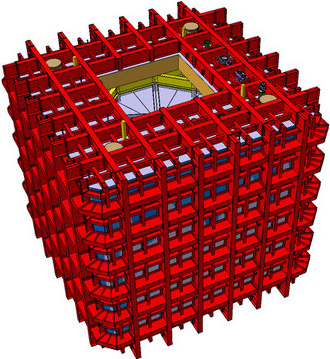
\includegraphics[width=0.80\textwidth]{./Figures/CryostatExterior.jpeg}
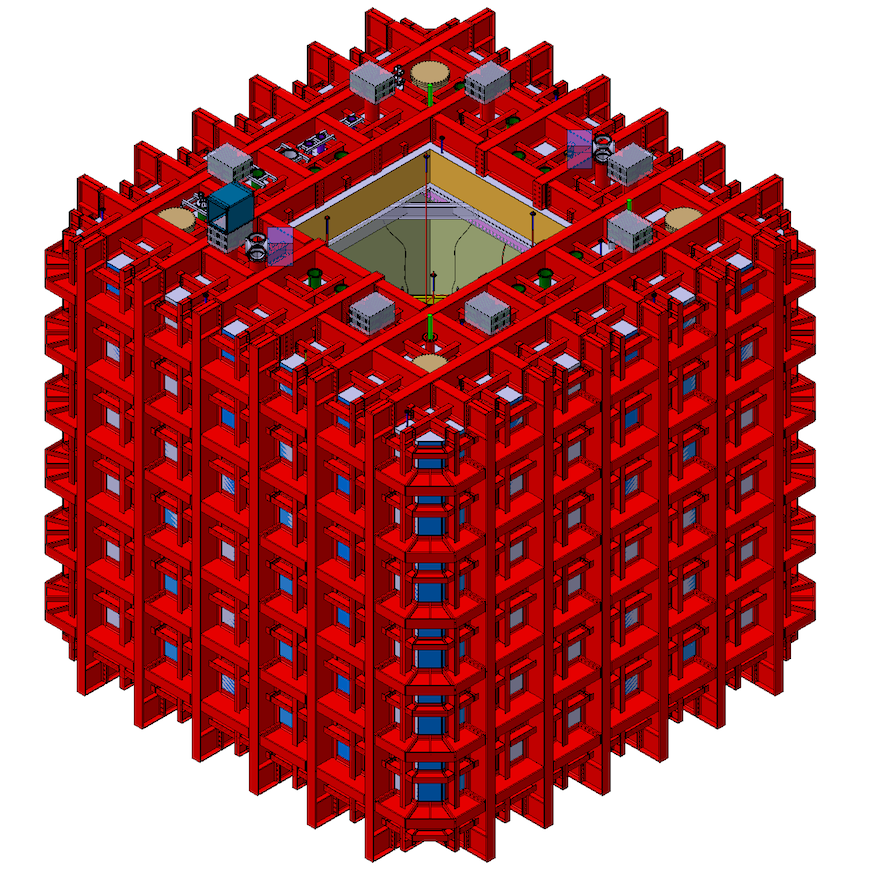
\includegraphics[height=0.6\textheight]{./Figures/cryostat_iso_crop.png}
\caption[3D view of the large \AAr\ cryostat]{3D conceptual external view of the \DSks\ \AAr\ cryostat.}
\label{fig:CryostatExternal}
\end{figure*}

\begin{figure*}[htbp]
%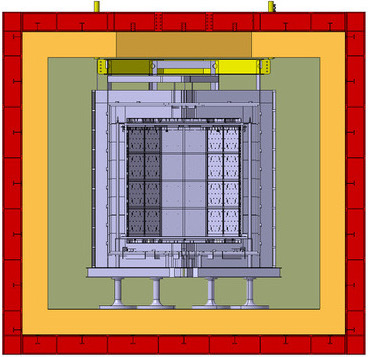
\includegraphics[width=\textwidth]{./Figures/Cryostat-InternalAssembly.jpeg}
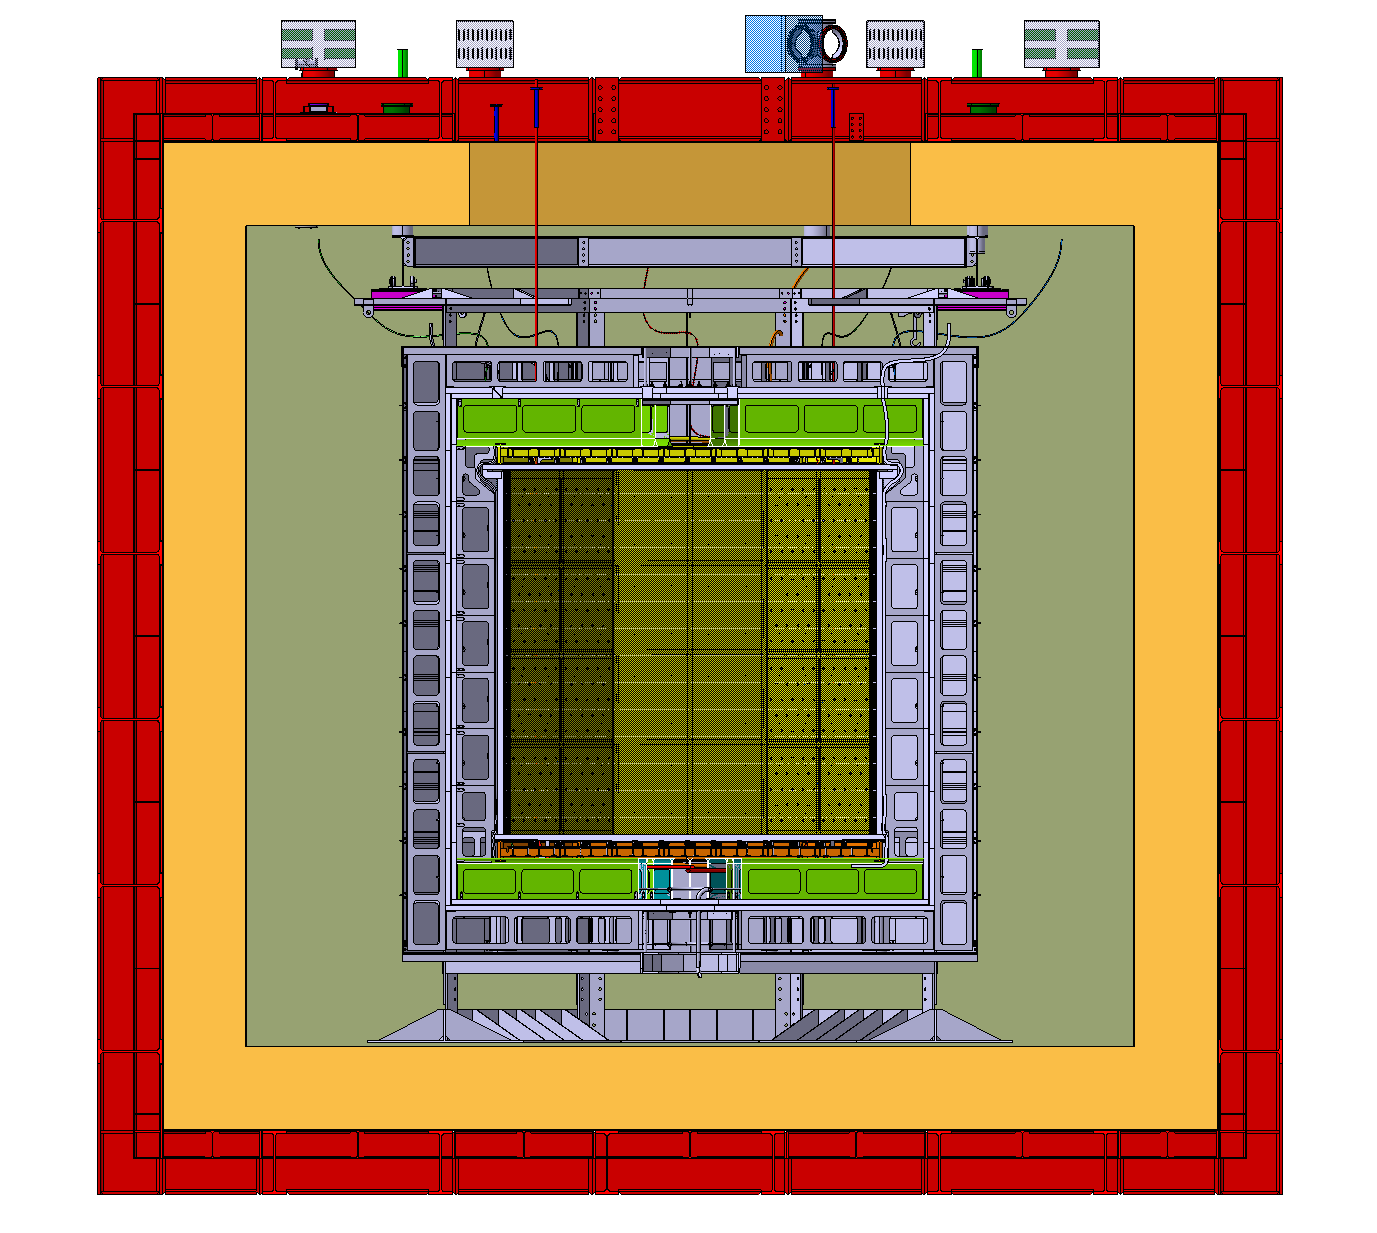
\includegraphics[height=0.6\textheight]{./Figures/cryostat_section_view_crop.png}
\caption[Cross-sectional view of the large \AAr\ cryostat]{Cross-sectional view of the large \AAr\ cryostat containing the \LArTPC\ and Veto detectors and showing the top-cap concept.}
\label{fig:CryostatAssembly}
\end{figure*}

%\begin{figure*}[!t]
%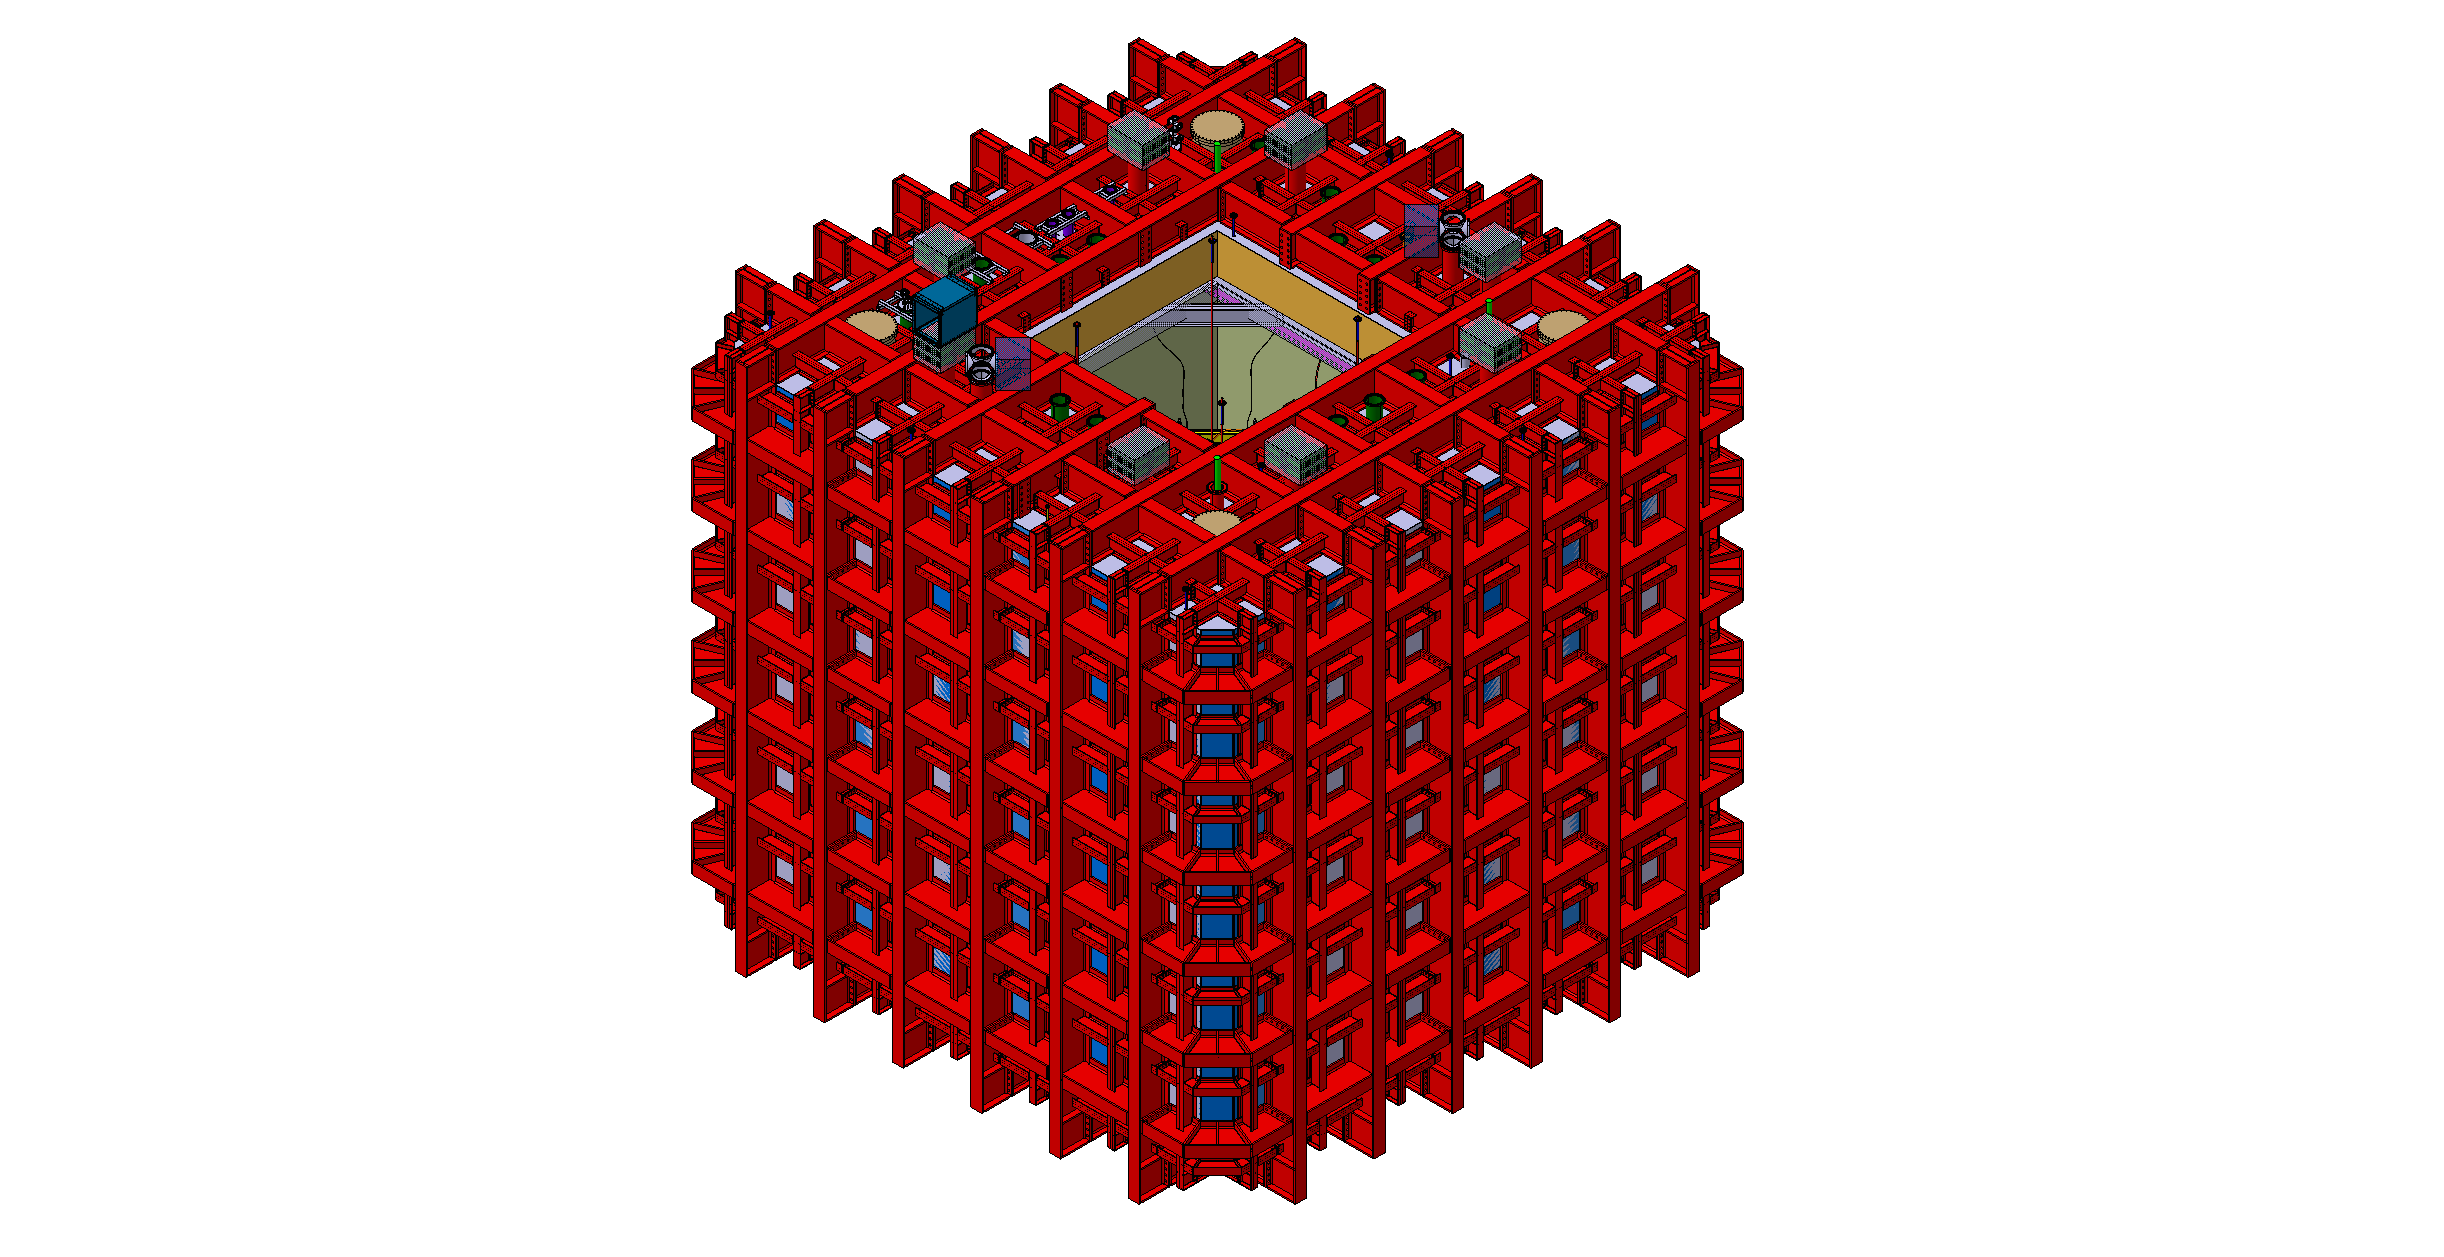
\includegraphics[height=0.45\textwidth]{./Figures/cryostat_iso.png}
%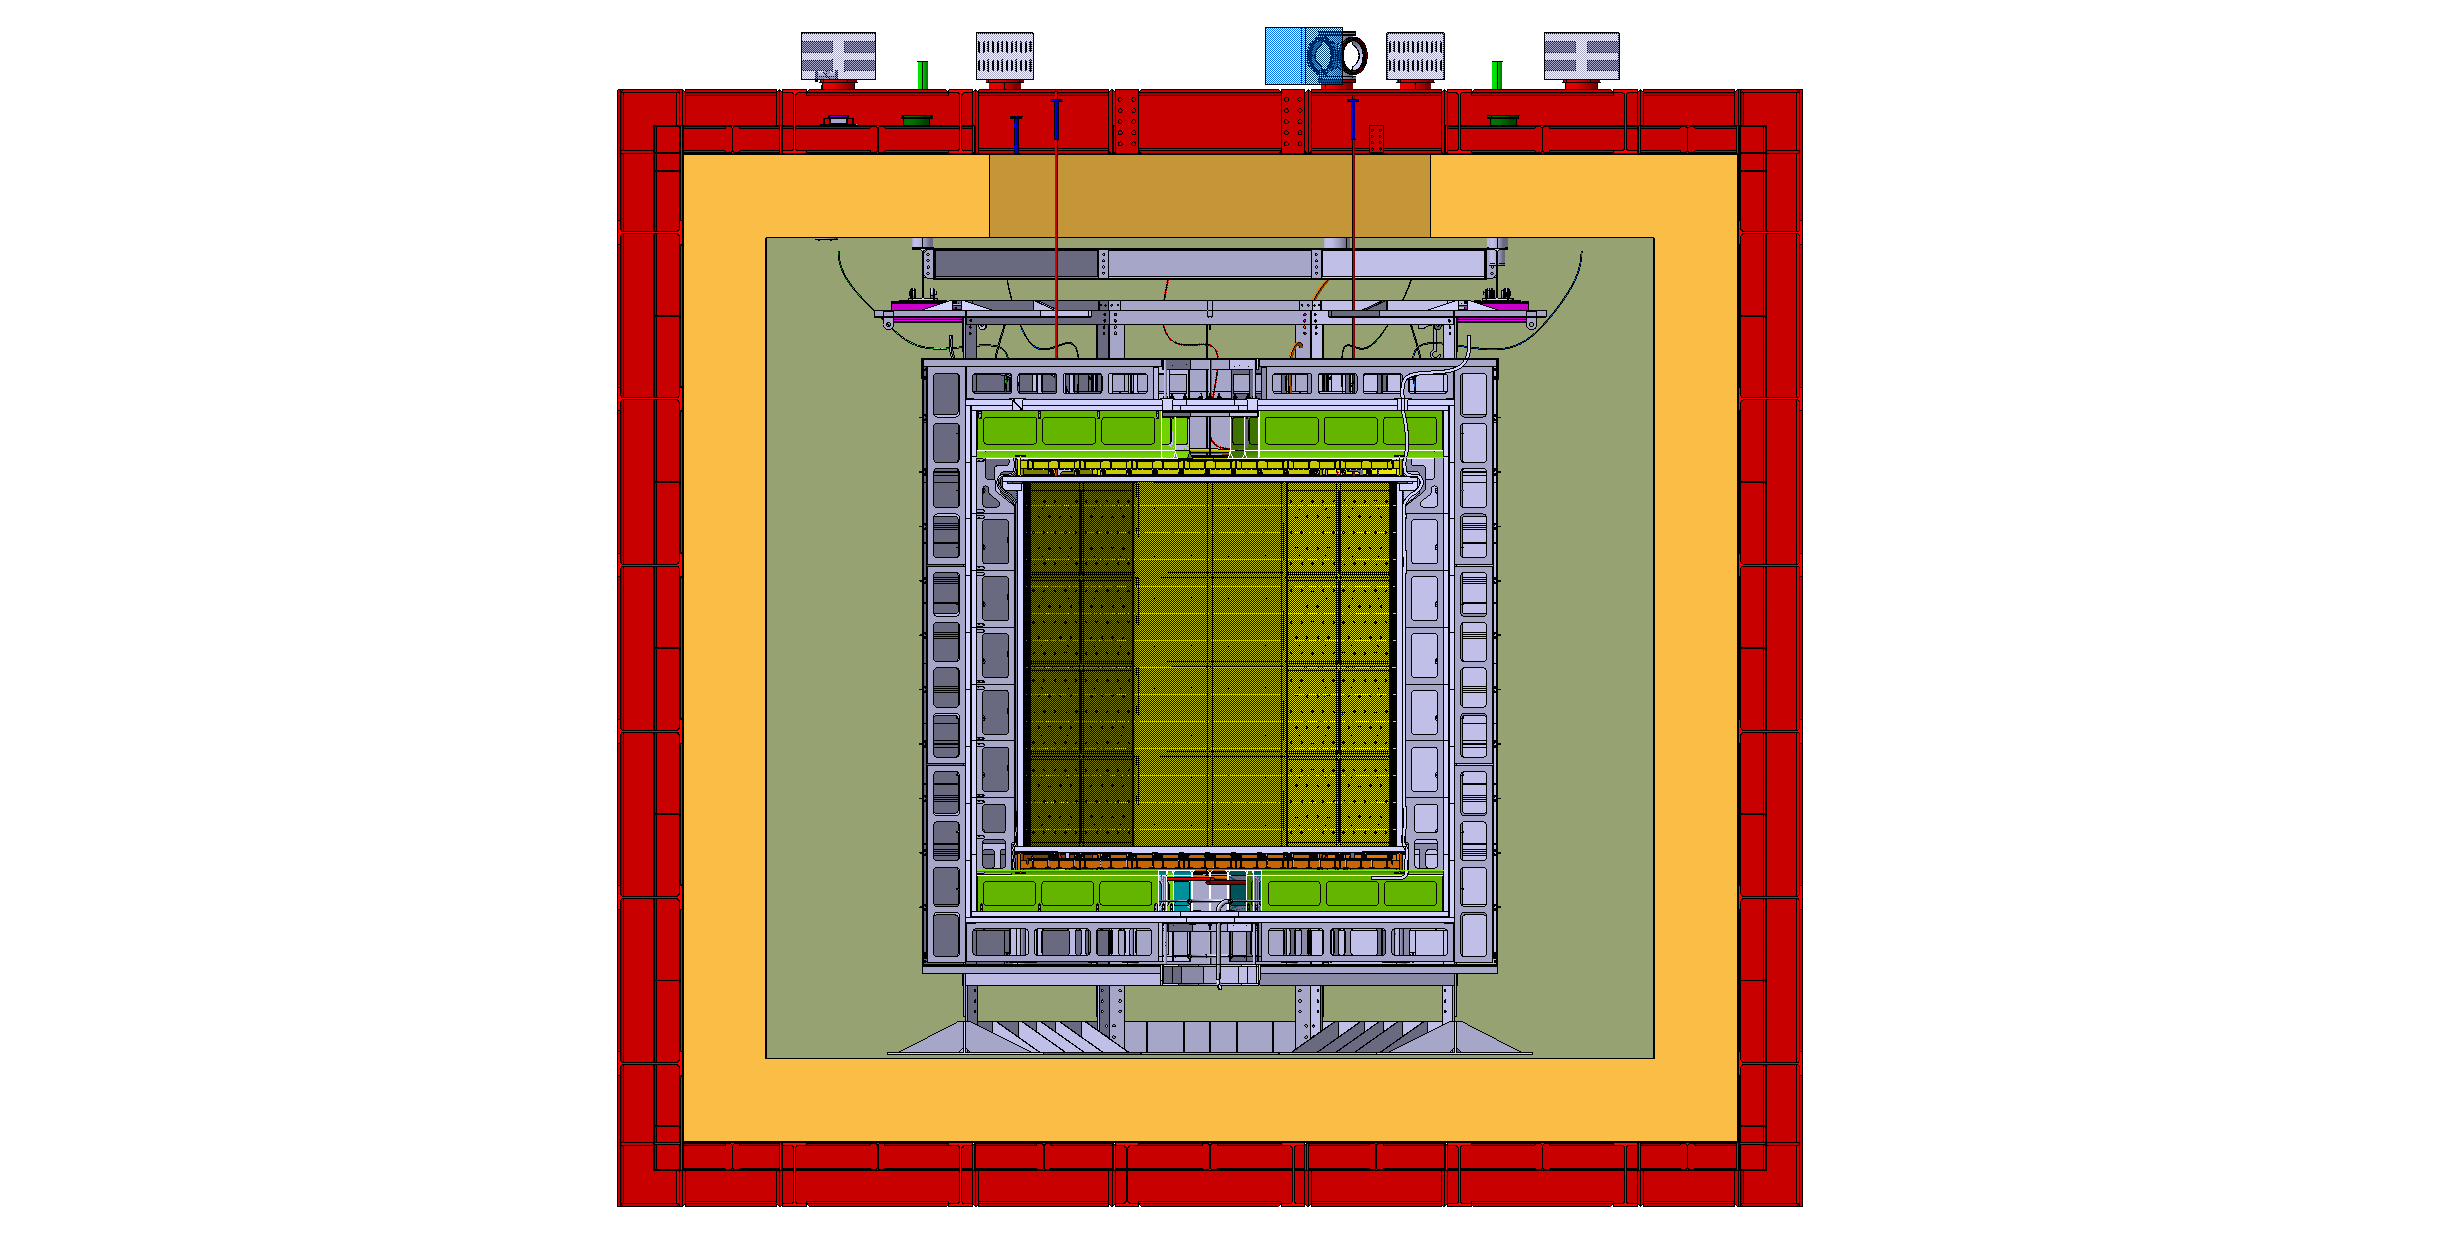
\includegraphics[height=0.45\textwidth]{./Figures/cryostat_section_view.png}
%\caption[3D and cross-sectional view of the large \AAr\ cryostat]{{\bf Top:} 3D cad view  view of the \DSks\ \AAr\ cryostat. {\bf Bottom:} Cross-sectional view of the large \AAr\ cryostat containing the \LArTPC\ and Veto detectors and showing the top-cap concept.}
%\label{fig:CryostatViews}
%\end{figure*}

Two cryostats of the same size as the one proposed here have been constructed at \CERN\ and one of them has been brought into operation in the second half of 2018. The experience gained there in the design, construction and operation will be fully translated to the \DSks\ project, through the involvement of the \CERN\ group that was responsible for the construction and operations of the \pDUNE\ cryostat. For that reason, the same mechanical constraints, dimension and thermal properties have been kept. The  \DSks\ cryostat is an improved version based on the experiences gained during the construction of the two \pDUNE\ cryostats, namely optimized fabrication and construction and access specific for \DSks\ project. A 3D conceptual view of the external part of the cryostat being planned for \DSks\ is shown in Figure~\ref{fig:CryostatExternal}. 

To make it as easy as possible for the access and support of the sub-systems of the \TPC\ and the Veto detectors, all components will now be inserted from the roof of the cryostat, with a ``closing cap'' concept being implemented. This has been previously deployed by the CERN team during other large-dual phase \TPC\ R\&D experiments and tested with the construction and operation of the first demonstrator for the \pDUNE\ project.  A cross-sectional view of the concept is shown in the right side of Figure~\ref{fig:CryostatAssembly}.  The plan is to assemble the bottom and sides of the Veto detector using a temporary support frame underneath the Veto detector, and then lower the TPC down into the Veto detector while it is attached to the closing cap, see Figure~\ref{fig:VetoAssembly}.  Once in place, the remaining parts of the Veto detector could be assembled, the entire detector system support transferred to the detector support system of the cryostat, and finally the temporary supports of the Veto detector that we required during construction removed.  At this point, the two detector volumes, that of the \TPC\ and that of the Veto, would be filled simultaneously such that the \LAr\ height in both volumes is equal at all times in order to reduce the mechanical stress on all of the detector components.

As mentioned in Sec.~\ref{sec:TPCCryo}, the \AAr\ cryogenics system will be built based on the combined experiences of the  \pDUNE\  cryogenics and the \DSfs\ cryogenics. The final optimization decision will be made taking into account that the different requirements of the \AAr\ cryostat for \DSks\ compared to those for \pDUNE, and the available space in Hall\,C of \LNGS. Penetrations on the roof of the cryostat are being finalized such to meet the requirements of the other sub-systems, as well as to provide the mechanical stability of the cryostat ceiling. The design and development plan will follow the successful experience of \pDUNE, with expert engineering assistance provided by the \CERN\ group, while already a firm baseline design is in place and schematically shown in the left side of Figure~\ref{fig:DSCryo}, along with the rest of the \DSks\ cryogenics system.